\documentclass[11pt]{article}

\usepackage[T1]{fontenc} % extended font encoding
\usepackage{enumerate} % lists
\renewcommand{\familydefault}{\sfdefault} % sans-serif
\usepackage{microtype} % better text justification
\usepackage{graphicx} % allow including pictures
\usepackage{color} % colors for pictures
\usepackage{textcomp} % for textminus
\usepackage{pagecolor} % background color for the first page
\usepackage{afterpage} % ditto ^^
\usepackage{tikz} % flow graph
\usetikzlibrary{dsp,chains}
\usepackage{parskip} % vertical paragraph spacing
\usepackage[a4paper, landscape, margin=1.5cm]{geometry} % basic geometry
\fboxsep=5mm % minibox spacing
\pagenumbering{gobble} % disable page numbering

% Style for a simple numbered list
\newenvironment{packed_enumerate}{
\begin{enumerate}
  \setlength{\itemsep}{1pt}
  \setlength{\parskip}{0pt}
  \setlength{\parsep}{0pt}
}{\end{enumerate}}

% Style for a roman literal numbered list
\newenvironment{packed_enumerate_i}{
\begin{enumerate}[I]
  \setlength{\itemsep}{1pt}
  \setlength{\parskip}{0pt}
  \setlength{\parsep}{0pt}
}{\end{enumerate}}


% Metadata
\pdfinfo{
   /Author (Zlosynth Instruments)
   /Title  (Kaseta - User Manual)
}

\begin{document}

% Front page should be black
\pagecolor{black}\afterpage{\nopagecolor}

% Front title
\title{\textcolor{white}{MANUAL}}
\author{}
\date{}

% Left column of the front page
\begin{minipage}{0.4\textwidth}
\color{white}
\maketitle

% Overview box
\noindent\colorbox{white}
{
\begin{minipage}{0.85\textwidth}\color{black}
Kaseta is a multi-purpose module inspired by reel-to-reel tape machines. It
simulates magnetic hysteresis to provide warm saturation, its four independent
delay lines can be used to sculpt rhythms or feedback loops, and it offers wow
and flutter control. The module also goes beyond typical tape machine features,
with free-moving delays, trigger sequencing, and an internal oscillator.
\end{minipage}
}

\vspace{1cm}

% Specs table
\begin{minipage}{0.8\textwidth}\color{white}
\begin{tabular}{@{}rl@{}}
  Width & 20 HP \\
  Depth & 28 mm \\
  % TODO: Needs to be re-measured
  Power & +12 V (85 mA), \textminus12 V (7 mA) \\
  Input impedance & 100 kΩ \\
  CV inputs & \textminus5 to +5 V, 16-bit, 2 kHz \\
  Trigger output & 0 to +5 V, 10 ms \\
  Audio & 24-bit, 48 kHz
\end{tabular}
\end{minipage}

\vspace{1cm}

% Features list
\begin{minipage}{0.8\textwidth}\color{white}
\begin{tabular}{@{}l}
  - Delay with 4 reading heads \\
  - Tape saturation simulation \\
  - Wow and flutter effects \\
  - Tone control \\
  - Trigger sequencing \\
  - Voltage-controlled oscillator \\
  - Stereo panning
\end{tabular}
\end{minipage}

\end{minipage}%
% Right column
\begin{minipage}{0.6\textwidth}
\vspace{8mm}

% Illustration of the panel
\begin{center}
  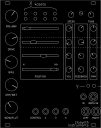
\includegraphics[width=0.8\textwidth]{schema.pdf}
\end{center}

\end{minipage}

% Start of the second page
\newpage
\color{black}

% Left column
\begin{minipage}[t]{0.35\textwidth}
\setlength{\parskip}{6pt}

\section{Installation}

Kaseta is 20 HP wide. It is powered by a +12V/{\textminus}12V 2\texttimes5
connector. The red stripe (\textminus12V) has to be connected on the side of the
board marked with the white line. The module must be mounted in a eurorack case.

\end{minipage}%
\begin{minipage}{0.05\textwidth}
\phantom{ }
\end{minipage}%
% Right column
\begin{minipage}[t]{0.55\textwidth}
\setlength{\parskip}{6pt}

\section{Controls, inputs and outputs}

Audio input, two outputs.

5 knobs on left.

2 speed and tone.

4 rows of identical pots controlling delay reading heads.

Control inputs than can be mapped to any of those attributes.

Display.

Button for tempo tap and access to alt attributes.

Y impulse, signalizing output of trigger sequencer IMPULSE.

\section{Mapping}

Each of the 4 multi-purpose control inputs can be mapped to any of the
knobs:

\begin{packed_enumerate}
  \item Plug a cable into one of the control inputs.
  \item Display will signalize mapping.
  \item Turn the desired target knob.
\end{packed_enumerate}

The mapping is persisted between restarts. Disconnect a cable to unmap it.

\section{Calibration}

Some of the attributes are following 1V/oct standard. To increase accuracy,
calibrate each of the control inputs.

\begin{packed_enumerate}
  \item While holding the button, connect a jack to an input.
  \item The first and second LED should light up.
  \item Play note C on the CV source and press the button.
  \item Now, the third and fourth LED should light up.
  \item Play C one octave higher and press the button again.
\end{packed_enumerate}

The calibration is persisted between restarts and disconnects.

\end{minipage}

\newpage

\section{Signal flow}

\vspace{2.5cm}
\begin{figure*}[ht]
    \center
    \begin{tikzpicture}
        \matrix (m1) [row sep=6mm, column sep=12mm]
        {
            &
            \node[dspnodeopen,dsp/label=above] (pre-amp-control)     {Pre-amp};     &
            &
            \node[dspnodeopen,dsp/label=above] (drive-bias-control)  {Drive+Bias};  &
            \node[dspnodeopen,dsp/label=above] (dry-wet-control)     {Dry/Wet};     &
            \node[dspnodeopen,dsp/label=above] (wow-flutter-control) {Wow/Flutter}; &
            \node[dspnodeopen,dsp/label=above] (tone-control)        {Tone};        &
            \\
            %-------------------------------------------------------------------
            \node[dspnodeopen,dsp/label=left] (input)             {Input};       &
            \node[dspmultiplier]              (pre-amp)           {};            &
            \node[dspnodefull]                (dry-wet-split)     {};            &
            \node[dspsquare]                  (hysteresis)        {Hysteresis};  &
            \node[dspmixer]                   (dry-wet-mix)       {};            &
            \node[dspsquare]                  (time-effect)       {Time effect}; &
            \node[dspsquare]                  (filter)            {Filter};      &
            \node[coordinate]                 (filter-to-write-a) {};            \\
            %-------------------------------------------------------------------
            &
            &
            \node[coordinate] (dry-wet-bypass-a) {}; &
            &
            \node[coordinate] (dry-wet-bypass-b) {}; &
            &
            &
            \\
            %-------------------------------------------------------------------
            \node[coordinate] (feedback-mixer-to-write) {};      &
            \node[dspsquare]  (write)                   {Write}; &
            &
            &
            &
            &
            &
            \node[coordinate] (route-to-write-b)        {};      \\
            %-------------------------------------------------------------------
            &
            \node[coordinate] (delay-nw) {}; &
            &
            &
            &
            &
            \node[coordinate] (delay-ne) {}; &
            \\
            %-------------------------------------------------------------------
            &
            \node[coordinate] (delay-sw)   {}; &
            &
            &
            &
            \node[coordinate] (read-point) {}; &
            \node[coordinate] (delay-se)   {}; &
            \\
            %-------------------------------------------------------------------
            \node[dspmixer]                    (feedback-mixer)         {};                   &
            &
            &
            &
            \node[dspmultiplier]               (feedback)               {};                   &
            \node[dspsquare]                   (read)                   {Read N};             &
            \node[dspnodeopen,dsp/label=right] (position-speed-control) {Position N / Speed}; \\
            %-------------------------------------------------------------------
            \node[dspnodefull,dsp/label=below] (other-feedback)     {\textit{Other heads}}; &
            &
            &
            &
            \node[dspnodeopen,dsp/label=below] (feedback-control)   {Feedback N};           &
            \node[dspmultiplier]               (volume-pan)         {};                     &
            \node[dspnodeopen,dsp/label=right] (volume-pan-control) {Volume N + Pan N};     \\
            %-------------------------------------------------------------------
            & & & & & & \\ % Spacing
            %-------------------------------------------------------------------
            &
            &
            &
            &
            &
            \node[dspmixer]                    (playback-mixer) {};                     &
            \node[dspnodefull,dsp/label=right] (other-playback) {\textit{Other heads}}; \\
            %-------------------------------------------------------------------
            &
            &
            &
            &
            &
            \node[dspnodeopen,dsp/label=below] (outputs) {Outputs}; &
            \\
            %---------------------------------------------------------------
            & & & & & & \\ % Spacing
        };
        % First row of flow
        \draw[dspflow]         (input) -- (pre-amp);
        \draw[dspflow]       (pre-amp) -- (dry-wet-split);
        \draw[dspflow] (dry-wet-split) -- (hysteresis);
        \draw[dspflow]    (hysteresis) -- (dry-wet-mix);
        \draw[dspflow]   (dry-wet-mix) -- (time-effect);
        \draw[dspflow]   (time-effect) -- (filter);

        % Controls
        \draw[dspconn]        (pre-amp-control) -- (pre-amp);
        \draw[dspconn]     (drive-bias-control) -- (hysteresis);
        \draw[dspconn]        (dry-wet-control) -- (dry-wet-mix);
        \draw[dspconn]    (wow-flutter-control) -- (time-effect);
        \draw[dspconn]           (tone-control) -- (filter);
        \draw[dspconn]     (volume-pan-control) -- (volume-pan);
        \draw[dspconn]       (feedback-control) -- (feedback);
        \draw[dspconn] (position-speed-control) -- (read);

        % Dry/wet bypass
        \draw[dspline]    (dry-wet-split) -- (dry-wet-bypass-a);
        \draw[dspflow] (dry-wet-bypass-a) -- (dry-wet-bypass-b);
        \draw[dspline] (dry-wet-bypass-b) -- (dry-wet-mix);

        % Route to the write head
        \draw[dspline]            (filter) -- (filter-to-write-a);
        \draw[dspline] (filter-to-write-a) -- (route-to-write-b);
        \draw[dspflow]  (route-to-write-b) -- (write);

        % Delay block
        \draw[line width=0.7mm] (delay-nw) -- (delay-sw) -- (delay-se) -- (delay-ne) -- cycle;

        % Writing and reading heads
        \draw[dspflow] (write) -- (delay-nw);
        \draw[dspflow] (read-point) -- (read);

        % Feedback flow
        \draw[dspflow]                    (read) -- (feedback);
        \draw[dspflow]                (feedback) -- (feedback-mixer);
        \draw[dspflow]          (feedback-mixer) -- (feedback-mixer-to-write);
        \draw[dspflow]          (other-feedback) -- (feedback-mixer);
        \draw[dspflow] (feedback-mixer-to-write) -- (write);

        % Playback flow
        \draw[dspflow]            (read) -- (volume-pan);
        \draw[dspflows]     (volume-pan) -- (playback-mixer);
        \draw[dspflows] (other-playback) -- (playback-mixer);
        \draw[dspflows] (playback-mixer) -- (outputs);
    \end{tikzpicture}
    \caption{\label{flowchart}{\it
      Signal flow within the module. Only a single reading head is shown for clarity.}}
\end{figure*}

\newpage

\section{Pre-amp}

What is the range. What is it good for. What signalizes clipping.

Nothing plugged in, use tone as amp, some other as frequency control, play sine on input.

\section{Saturation}

About the maths behind, what it does on real tape.

Image of what happens to the sound.

Explanation of bias.

Explanation of the sweet spot with pre-amp.

Bias is most pronounced on weak input signal without distortion.

Danger zone.

\section{Delay}

Heads. Feedback vs blend. Ranges. Clock in. Gate out.

Longest delay is. Switchable ranges.

Image illusatration of the signal flow.

Switch to make volume a chance for the gate.

Tap-in, regular or clock signal in mapped control.

Image 

How to recover from feedback loop.

\section{Tone}

Images with low-pass, all-pass, high-pass positions.

Explanation on how it is applied per head.

Mention of the switch setting it for feedback/all.

\section{Wow and flutter}

Wow: Oscillation or change in pitch, caused by warped tape, low frequency, <4Hz

Flutter: Simulates scratched tape or friction, causes inconsistent information, vibration in frequency spectrum, high frequency, >4Hz

\section{Compression}

Explanation of what happens with output (saturation). Also can enable compression instead, using switch.

\section{Options}

Delay echo vs. audio rate
Quantization 1/8
Quantization 1/6
Wow cyclic vs. random
Flutter cyclic vs. random
Danger zone
Rewind/speed

\newpage

\section{Patch book}

Some basic combinations to get you started. TODO: Custom wow/flutter using position modulation.

\vspace{5mm}
\noindent
\begin{minipage}[t]{0.45\textwidth}

\subsection{Warm saturation}

\vspace{5mm}
\begin{center}
  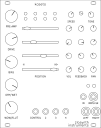
\includegraphics[width=0.7\textwidth]{schema-inverted.pdf}
\end{center}

* Basic hysteresis.
* Warm soft saturation on piano is nice.

\end{minipage}%
\begin{minipage}{0.05\textwidth}
\phantom{ }
\end{minipage}%
% Right column
\begin{minipage}[t]{0.45\textwidth}
\subsection{Wow and flutter}

\vspace{5mm}
\begin{center}
  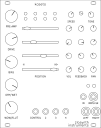
\includegraphics[width=0.7\textwidth]{schema-inverted.pdf}
\end{center}

Find a better name.

* Basic flutter with disabled hysteresis.
\end{minipage}

\newpage


\subsection{Simple echo}

* Basic evenly spread one time delay.

\subsection{Feedback pads}

* Basic feedback delay. Single head, slightly delayed.

\subsection{Comb filter}

* Audio level delay. Just one slightly delayed head playing and feeding back.
  Perhaps on specific tones.

\subsection{Thickiening of basic sine}

* Plain sine. All four heads playing in a small distance from each other.
  Producing reverb. Add flutter to make it forever moving and changing.

\subsection{Tremolo}

* Basic tremolo, just cyclic flutter.

\subsection{Rhytmical echo}

* Delays comming back, with some heads close, some far to repeat way later.

\subsection{Rhythm sequencer}

* Percussion rhythm.

\subsection{Almost sidechaining}

* When bass drum and single oscillator tone play at the same time with high
  saturation and low bias, it works like sidechaining.

\subsection{Cutting cymbals}

* Short cybmals, low bias cuts weak signal.

\subsection{Ping pong echo}

* Ping pong snare. Like Daughter's New Ways.

\subsection{Samples from the past}

* With non-warping delay, CV S and H input to delay value, selecting samples from
  the past.

\subsection{Rewind}

* Playing a mellow song, slow speed. Fading when approaching end, switch to another head.

\subsection{Distortion unchained}

* Hardcore distortion

\newpage





\noindent
% NOTE: Configuration is not exposed yet.
% \begin{minipage}[t]{0.3\textwidth}
% \section{Configuration}
% \end{minipage}%
% \begin{minipage}{0.05\textwidth}
% \phantom{ }
% \end{minipage}%
% % Center column
% NOTE: This will be introduced with the first patch release.
% \begin{minipage}[t]{0.3\textwidth}
% \section{Changelog}
% \end{minipage}
% \begin{minipage}{0.05\textwidth}
% \phantom{ }
% \end{minipage}%
% Right column
\begin{minipage}[t]{0.3\textwidth}
\section{Questions?}

\begin{center}
petr@zlosynth.com
\end{center}
\end{minipage}

\end{document}
